% # 8.4 设计并发代码的注意事项

我们已经看到了很多为线程分配工作的方法和影响性能的因素,以及这些因素是如何影响选择数据访问模式和数据结构的。虽然,有很多设计并发代码的内容,但还需要考虑的更多,比如异常安全和可扩展性。随着核数的增加,性能越来越高(无论是在减少执行时间,还是增加吞吐率),这样的代码称为“可扩展”代码。理想状态下,性能随着核数的增加线性增长,也就是当系统有100个处理器时,其性能是系统只有1核时的100倍。

虽然,非扩展性代码依旧可以正常工作——单线程应用就无法扩展,例如:异常安全是一个正确性问题,如果代码不是异常安全的,最终会破坏不变量,或是造成条件竞争,亦或是操作抛出异常意外终止应用。我们就先来看一下异常安全的问题。

\mySubsubsection{8.4.1}{并行算法中的异常安全}

异常安全是衡量C++代码很重要的指标,并发代码也不例外。实际上,相较于串行算法,并行算法常会更注意异常问题。操作在串行算法中抛出异常时,算法只需要对其本身进行处理,就可以避免资源泄露和损坏不变量,这里允许异常传递给调用者,由调用者对异常进行处理。在并行算法中很多操作要运行在独立的线程上,所以就不能传播异常。如果函数在创建新线程后异常退出,那么应用会终止。

让我们回顾一下代码2.8中的parallel\_accumulate函数:

代码8.2 \texttt{std::accumulate}的原始并行版本(源于代码2.8)

\begin{cpp}
template<typename Iterator,typename T>
struct accumulate_block
{
  void operator()(Iterator first,Iterator last,T& result)
  {
    result=std::accumulate(first,last,result);  // 1
  }
};

template<typename Iterator,typename T>
T parallel_accumulate(Iterator first,Iterator last,T init)
{
  unsigned long const length=std::distance(first,last);  // 2

  if(!length)
    return init;

  unsigned long const min_per_thread=25;
  unsigned long const max_threads=
    (length+min_per_thread-1)/min_per_thread;

  unsigned long const hardware_threads=
    std::thread::hardware_concurrency();

  unsigned long const num_threads=
    std::min(hardware_threads!=0?hardware_threads:2,max_threads);

  unsigned long const block_size=length/num_threads;

  std::vector<T> results(num_threads);  // 3
  std::vector<std::thread> threads(num_threads-1);  // 4

  Iterator block_start=first;  // 5
  for(unsigned long i=0;i<(num_threads-1);++i)
  {
    Iterator block_end=block_start;  // 6
    std::advance(block_end,block_size);
    threads[i]=std::thread(  // 7
      accumulate_block<Iterator,T>(),
      block_start,block_end,std::ref(results[i]));
    block_start=block_end;  // 8
  }
  accumulate_block()(block_start,last,results[num_threads-1]);  // 9

  std::for_each(threads.begin(),threads.end(),
    std::mem_fn(&std::thread::join));

  return std::accumulate(results.begin(),results.end(),init);  // 10
}
\end{cpp}

看一下异常在哪抛出:在调用函数的地方或在用户定义类型上执行某个操作时抛出异常。

首先,distance②会对用户定义的迭代器进行操作。这时还没有做任何事情,所以对于调用线程来说一切安好,接下来就需要分配results③和threads④。再后,调用线程依旧没有做任何事情或产生新线程,所以这里也没有问题。当然,在构造threads抛出异常时,析构函数会将已分配的results进行清理。

跳过block\_start⑤的初始化(因为也是安全的),来到了产生新线程的循环⑥⑦⑧。在⑦处创建了第一个线程,如果再抛出异常就会出问题,新的\texttt{std::thread}对象将会销毁,程序将调用\texttt{std::terminate}来中断程序的运行。

使用\texttt{std::terminate}的地方,可不是什么好地方。

accumulate\_block⑨的调用就可能抛出异常,就会产生和上面类似的结果,线程对象将会销毁,并调用\texttt{std::terminate}。另一方面,调用\texttt{std::accumulate}⑩可能会抛出异常,不过处理起来没什么难度,因为所有的线程在这里已经汇回主线程了。

上面只是对主线程来说的,不过还有很多地方会抛出异常:调用accumulate\_block的新线程就会抛出异常①。没有任何catch块,所以不会处理这个异常,并且当异常发生时会调用\texttt{std::terminater()}来终止应用。

也许这里的异常问题并不明显,不过这段代码是非异常安全的。

\textbf{添加异常安全}

已经确定了所有抛出异常的地方,并且了解了异常所带来的后果。接着,就让我们解决一下在新线程上的异常问题。

如果仔细了解过新线程用来完成什么样的工作,要返回一个计算的结果的同时,允许代码产生异常,可以将\texttt{std::packaged\_task}和\texttt{std::future}结合使用。如果使用\texttt{std::packaged\_task}重新构造代码,可能会是如下模样。

代码8.3 使用\texttt{std::packaged\_task}的并行\texttt{std::accumulate}

\begin{cpp}
template<typename Iterator,typename T>
struct accumulate_block
{
  T operator()(Iterator first,Iterator last)  // 1
  {
    return std::accumulate(first,last,T());  // 2
  }
};

template<typename Iterator,typename T>
T parallel_accumulate(Iterator first,Iterator last,T init)
{
  unsigned long const length=std::distance(first,last);

  if(!length)
    return init;

  unsigned long const min_per_thread=25;
  unsigned long const max_threads=
    (length+min_per_thread-1)/min_per_thread;

  unsigned long const hardware_threads=
    std::thread::hardware_concurrency();

  unsigned long const num_threads=
    std::min(hardware_threads!=0?hardware_threads:2,max_threads);

  unsigned long const block_size=length/num_threads;

  std::vector<std::future<T> > futures(num_threads-1);  // 3
  std::vector<std::thread> threads(num_threads-1);

  Iterator block_start=first;
  for(unsigned long i=0;i<(num_threads-1);++i)
  {
    Iterator block_end=block_start;
    std::advance(block_end,block_size);
    std::packaged_task<T(Iterator,Iterator)> task(  // 4
      accumulate_block<Iterator,T>());
    futures[i]=task.get_future();  // 5
    threads[i]=std::thread(std::move(task),block_start,block_end);  // 6
    block_start=block_end;
  }
  T last_result=accumulate_block()(block_start,last);  // 7

  std::for_each(threads.begin(),threads.end(),
    std::mem_fn(&std::thread::join));

  T result=init;  // 8
  for(unsigned long i=0;i<(num_threads-1);++i)
  {
    result+=futures[i].get();  // 9
  }
  result += last_result;  // 10
  return result;
}
\end{cpp}

第一个修改就是对accumulate\_block的调用,现在直接将结果返回,而不是使用引用将结果存储在某个地方①。\texttt{std::packaged\_task}和\texttt{std::future}是线程安全的,所以可以用来对结果进行转移。当调用\texttt{std::accumulate}②时,需要显式传入T的默认构造函数,而非复用result的值。

下一个改动就是,不用vector来存储结果,而使用future vector为每个新生线程存储\texttt{std::future<T>}③。新线程生成的循环中,首先要为accumulate\_block创建一个任务④。\texttt{std::packaged\_task<T(Iterator,Iterator)>}需要操作的两个Iterator和T。然后,从任务中获取future⑤,再将需要处理的数据块的开始和结束信息传入⑥,让新线程去执行这个任务。任务执行时,future会获取结果或抛出异常。

使用future就不能获得结果数组,所以需要将最终数据块的结果赋给变量进行保存⑦,而非对数组进行填槽。同样,因为要从future中获取结果,使用简单的for循环,就要比使用\texttt{std::accumulate}好的多。循环从提供的初始值开始⑧,并且将每个future上的值进行累加⑨。如果相关任务抛出异常就会捕捉到,并且使用get()的时候获取数据时,这个异常会再次抛出。最后,在返回结果之前,将最后一个数据块上的结果添加入结果中⑩。

这样问题就解决了:工作线程上抛出的异常,可以在主线程上抛出。如果不止一个工作线程抛出异常,那么只有一个异常能在主线程中抛出。如果这个问题很重要,可以使用类似\texttt{std::nested\_exception}对所有抛出的异常进行捕捉。

剩下的问题:当第一个新线程和当所有线程都汇入主线程时抛出异常时,就会让线程产生泄露。最简单的方法就是捕获所有抛出的线程,汇入的线程依旧是joinable()的,并且会再次抛出异常:

\begin{cpp}
try
{
  for(unsigned long i=0;i<(num_threads-1);++i)
  {
    // ... as before
  }
  T last_result=accumulate_block()(block_start,last);

  std::for_each(threads.begin(),threads.end(),
  std::mem_fn(&std::thread::join));
}
catch(...)
{
  for(unsigned long i=0;i<(num_thread-1);++i)
  {
  if(threads[i].joinable())
    thread[i].join();
  }
  throw;
}
\end{cpp}

现在好了,无论线程如何离开这段代码都可以汇入,可以将“正常”控制流上的线程,以及在\textit{catch}块上执行的线程进行汇入。不过,\textit{try-catch}很不美观,并且有重复代码。重复代码是没有必要的,因为这就意味着更多的地方需要改变。现在让我们来提取一个对象的析构函数,看一下类实现:

\begin{cpp}
class join_threads
{
  std::vector<std::thread>& threads;
public:
  explicit join_threads(std::vector<std::thread>& threads_):
    threads(threads_)
  {}
  ~join_threads()
  {
    for(unsigned long i=0;i<threads.size();++i)
    {
      if(threads[i].joinable())
        threads[i].join();
    }
  }
};
\end{cpp}

除了使用向量的方式扩展线程量,这个类和在代码2.3中看到的thread\_guard类很相似。简化后的代码如下所示:

代码8.4 异常安全版\texttt{std::accumulate}

\begin{cpp}
template<typename Iterator,typename T>
T parallel_accumulate(Iterator first,Iterator last,T init)
{
  unsigned long const length=std::distance(first,last);

  if(!length)
    return init;

  unsigned long const min_per_thread=25;
  unsigned long const max_threads=
    (length+min_per_thread-1)/min_per_thread;

  unsigned long const hardware_threads=
    std::thread::hardware_concurrency();

  unsigned long const num_threads=
    std::min(hardware_threads!=0?hardware_threads:2,max_threads);

  unsigned long const block_size=length/num_threads;

  std::vector<std::future<T> > futures(num_threads-1);
  std::vector<std::thread> threads(num_threads-1);
  join_threads joiner(threads);  // 1

  Iterator block_start=first;
  for(unsigned long i=0;i<(num_threads-1);++i)
  {
    Iterator block_end=block_start;
    std::advance(block_end,block_size);
    std::packaged_task<T(Iterator,Iterator)> task(
      accumulate_block<Iterator,T>());
    futures[i]=task.get_future();
    threads[i]=std::thread(std::move(task),block_start,block_end);
    block_start=block_end;
  }
  T last_result=accumulate_block()(block_start,last);
  T result=init;
  for(unsigned long i=0;i<(num_threads-1);++i)
  {
    result+=futures[i].get();  // 2
  }
  result += last_result;
  return result;
}
\end{cpp}

创建了线程容器,对新类型创建实例①,可让退出线程进行汇入。然后,可以在汇入循环中将线程删除,原理上说是安全的:因为线程无论怎么样退出,都需要汇入主线程。需要注意的是,对futures[i].get()②的调用会阻塞线程,直到结果准备就绪,所以不需要显式的将线程进行汇入。和代码8.2中不同:原始代码中需要将线程汇入,以确保results正确填充。不仅需要异常安全的代码,还需要较短的函数实现,而这里已经将汇入部分放到新(可复用)类型中去了。

\textbf{std::async()的异常安全}

当需要管理线程时,需要代码是异常安全的。那现在来看一下使用\texttt{std::async()}是怎样完成异常安全的。本例中标准库对线程进行了较好的管理,并且当future处以就绪状态时,就能生成新的线程。对于异常安全,还需要注意一件事,如果没有等待的情况下对future实例进行销毁,析构函数会等待对应线程执行完毕后才执行。这就能体现线程泄露的问题,因为线程还在执行,且持有数据引用。下面将展示使用\texttt{std::async()}完成异常安全的实现。

代码8.5 异常安全并行版\texttt{std::accumulate}——使用\texttt{std::async()}

\begin{cpp}
template<typename Iterator,typename T>
T parallel_accumulate(Iterator first,Iterator last,T init)
{
  unsigned long const length=std::distance(first,last);  // 1
  unsigned long const max_chunk_size=25;
  if(length<=max_chunk_size)
  {
    return std::accumulate(first,last,init);  // 2
  }
  else
  {
    Iterator mid_point=first;
    std::advance(mid_point,length/2);  // 3
    std::future<T> first_half_result=
      std::async(parallel_accumulate<Iterator,T>,  // 4
        first,mid_point,init);
    T second_half_result=parallel_accumulate(mid_point,last,T());  // 5
    return first_half_result.get()+second_half_result;  // 6
  }
}
\end{cpp}

这个版本是对数据进行递归划分,而非在预计算后对数据进行分块。因此,这个版本要比之前简单很多,并且这个版本也是异常安全的。和之前一样,要确定序列的长度①,如果其长度小于数据块包含数据的最大值,可以直接调用\texttt{std::accumulate}②。如果元素的数量超出了数据块包含数据的最大值,就需要找到数量中点③,将这个数据块分成两部分,然后再生成一个异步任务对另一半数据进行处理④。第二半的数据是通过直接的递归调用来处理的⑤,之后将两个块的结果加和到一起⑥。标准库能保证\texttt{std::async}的调用能够充分的利用硬件线程,并且不会产生线程的超额申请,一些“异步”调用在get()⑥后同步执行。

优雅的地方不仅在于利用硬件并发的优势,还能保证异常安全。如果有异常在递归⑤中抛出,通过\texttt{std::async}④所产生的future,将异常在传播时销毁。这就需要依次等待异步任务的完成,因此也能避免悬空线程的出现。另外,当异步任务抛出异常,且被future所捕获后,在对get()⑥调用的时候,future中存储的异常会再次抛出。

除此之外,设计并发代码还要考虑哪些其他因素?\textit{扩展性} (scalability)。随着系统中核数的增加,应用性能如何提升?

\mySubsubsection{8.4.2}{可扩展性和Amdahl定律}

扩展性代表了应用利用系统中处理器执行任务的能力。一种极端的方式就是将应用写死为单线程运行,这种应用就是完全不可扩展的。即使添加了100个处理器到你的系统中,应用的性能都不会有任何改变。另一种就是像SETI@Home\footnote[3]{\url{http://setiathome.ssl.berkeley.edu/}}项目一样,让应用使用系统中成千上万的处理器(以个人电脑的形式加入网络的用户)成为可能。

对于任意的多线程程序,运行时的工作线程数量会有所不同。应用初始阶段只有一个线程,之后会在这个线程上衍生出新的线程。理想状态:每个线程都做着有用的工作,不过这种情况几乎是不可能发生的。线程通常会花时间进行互相等待,或等待I/O操作的完成。

一种简化的方式就是就是将程序划分成“串行”和“并行”部分。串行部分:只能由单线程执行一些工作的地方。并行部分:可以让所有可用的处理器一起工作的部分。当在多处理系统上运行应用时,“并行”部分理论上会完成的相当快,因为其工作被划分为多份,放在不同的处理器上执行。“串行”部分则不同,只能一个处理器执行所有工作。这样的(简化)假设下,就可以随着处理数量的增加,估计一下性能的增益:当程序“串行”部分的时间用fs来表示,那么性能增益(P)就可以通过处理器数量(N)进行估计:

% ![](../../images/chapter8/amdahl\_law.png)
\begin{center}
  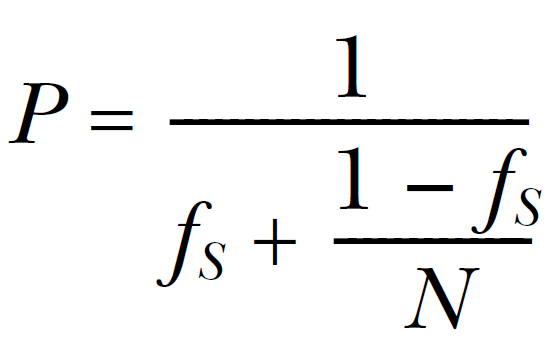
\includegraphics[width=0.7\textwidth]{content/chapter08/images/amdahl_law.png}\\
  图 8.2 递归划分数据
\end{center}

这就是Amdahl定律,讨论并发程序性能的时候都会引用到的公式。如果每行代码都能并行化,串行部分就为0,性能增益就为N。或者,当串行部分为1/3时,当处理器数量无限增长,都无法获得超过3的性能增益。

Amdahl定律明确了,对代码最大化并发可以保证所有处理器都能用来做有用的工作。如果将“串行”部分的减小,或者减少线程的等待,就可以在多处理器的系统中获取更多的性能收益。或者,当能提供更多的数据让系统进行处理,并且让并行部分做最重要的工作,就可以减少“串行”部分,以获取更高的性能增益。

扩展性:当有更多的处理器加入时,减少单个动作的执行时间,或在给定时间内做更多工作。有时这两个指标是等价的(如果处理器的速度相当快,就可以处理更多的数据)。选择线程间的工作划分的技术前,需要辨别哪些方面是能够扩展的。

本节开始已经提到,线程并非任何时候都做的是有用的工作。有时也会等待其他线程,或者等待I/O完成,亦或是等待其他事情。如果线程等待时,系统中还有必要的任务需要完成,就可以将等待“隐藏”起来。

\mySubsubsection{8.4.3}{使用多线程隐藏延迟}

之前讨论了很多有关多线程性能的话题。现在假设,线程在一个处理器上运行时不会偷懒,并且做的工作都很有用。然而实际应用中,线程会经常因为等待某些事情而阻塞。

不论等待的理由是什么,线程阻塞就意味着在等待CPU时间片。处理器将会在阻塞的时间内运行另一个线程,而不是什么事情都不做。因此,当知道一些线程需要耗费相当一段时间进行等待时,可以利用CPU的空闲时间去运行一个或多个线程。

试想一个病毒扫描程序,使用流水线对线程间的工作进行划分。第一个线程对文件系统进行检查,并将它们放入一个队列中。同时,另一个线程从队列中获取文件名,加载文件,之后进行病毒扫描。线程对文件系统中的文件进行扫描就会受到I/O操作的限制,所以可以通过执行额外的扫描线程,充分利用CPU的“空闲”时间。这时还需要一个文件搜索线程,以及足够多的扫描线程。当扫描线程为了扫描文件,还要从磁盘上读取到重要部分的文件时,就能体会到多扫描线程的意义所在了。不过,某些时候线程会过多,系统将会因为越来越多的任务切换而降低效率,就像8.2.5节描述的那样。

同之前一样,这也是一种优化,对修改(线程数量)前后性能的测量很重要。

应用可能不用额外的线程,而使用CPU的空闲时间。例如,如果线程因为I/O操作阻塞,这个线程可能会使用异步I/O(如果可以用的话),当I/O操作在后台执行完成后,线程就可以做工作了。其他情况下,一个线程等待其他线程去执行一个操作时,比起阻塞,不如让阻塞线程自己来完成这个操作,就像在第7章中看到的无锁队列那样。一个极端的例子中,当一个线程等待任务完成,并且这个任务还没有被其他任何线程所执行时,等待线程就可以执行这个任务,或执行另一个不完整的任务。代码8.1中排序函数会持续的对数据进行排序,即使那些数据已经不需要排序了。

比起添加线程数量对处理器进行充分利用外,有时也要在增加线程确保外部事件能够及时的响应,以提升系统的响应能力。

\mySubsubsection{8.4.4}{使用并发提高响应能力}

很多流行的图形化用户接口框架都是\textit{事件驱动型}(event driven),对图形化接口进行操作是通过按下按键或移动鼠标进行。为了确定所有事件和信息都能被正确的处理,应用通常会有一个事件循环,就像下面的代码:

\begin{cpp}
while(true)
{
  event_data event=get_event();
  if(event.type==quit)
    break;
  process(event);
}
\end{cpp}

显然,API中的细节可能不同,不过结构通常是一样的:等待一个事件,对其做必要的处理,之后等待下一个事件。如果是单线程应用,就会让长期任务很难执行完成。为了确保用户输入能得到及时的处理,无论应时在做些什么,get\_event()和process()必须以合理的频率调用。这就意味着任务需要周期性的悬挂,并且返回到事件循环中,get\_event()/process()必须在合适的地方进行调用,且每个选项的复杂程度取决于任务的实现方式。

通过使用并发分离关注点,可以将一个很长的任务交给一个全新的线程,并且留下一个专用的GUI线程来处理这些事件。线程可以通过简单的机制进行通讯,而不是将事件处理代码和任务代码混在一起。

代码8.6 将GUI线程和任务线程进行分离

\begin{cpp}
std::thread task_thread;
std::atomic<bool> task_cancelled(false);

void gui_thread()
{
  while(true)
  {
    event_data event=get_event();
    if(event.type==quit)
      break;
    process(event);
  }
}

void task()
{
  while(!task_complete() && !task_cancelled)
  {
    do_next_operation();
  }
  if(task_cancelled)
  {
    perform_cleanup();
  }
  else
  {
    post_gui_event(task_complete);
  }
}

void process(event_data const& event)
{
  switch(event.type)
  {
  case start_task:
    task_cancelled=false;
    task_thread=std::thread(task);
    break;
  case stop_task:
    task_cancelled=true;
    task_thread.join();
    break;
  case task_complete:
    task_thread.join();
    display_results();
    break;
  default:
    //...
  }
}
\end{cpp}

通过这种方式对关注点进行分离,用户线程将能及时的对事件进行响应。使用应用的时候,响应事件通常也是影响用户体验的重要一点,不恰当的执行特定操作(无论是什么操作),会让应用锁住。通过专门的事件处理线程,GUI就能处理指定的信息(比如对于调整窗口的大小或颜色,且不需要中断处理器,进行耗时的处理),还能向长期任务传递相关的信息。

现在,可以将本章中在设计并发代码时要考虑的问题进行一下回顾。作为一个整体,它们都具有代表性,不过当你熟练的使用“多线程编程”时,考虑其中的很多问题将变成习惯。如果你是初学者,我希望这些例子能让你明白,这些问题是如何影响多线程代码的。

% ------------

% [3] http://setiathome.ssl.berkeley.edu/